\section{RationalGRL Methodology and Metamodel}
\label{sect:overview}

In this section we present a high-level overview of the RationalGRL framework. In the first subsection, we present a methodology, specifying how practitioners can use RationalGRL to create goal models with traceability links to underlying arguments. In the second subsection, we link the new argumentation elements and relations to the existing elements and relations of GRL in a metamodel. This metamodel serves as the specification for an implementation. In Section~\ref{sect:tool} we briefly discuss our prototype implementation based on this metamodel.

\subsection{RationalGRL Methodology} 

As mentioned in Section~\ref{sect:introduction}, the RationalGRL framework uses concepts from practical reasoning argument scheme (PRAS) to help integrating goal models with the detailed discussions and arguments the stakeholders pose during the analysis phase. That is, the RationalGRL framework includes two main parts: Argumentation modeling and GRL modeling. 

For the GRL part, we first need to create the ``initial'' GRL model by analyzing the non-functional requirements in the requirements specification document and by refining the high-level goals into operationalized tasks. For the argumentation part, arguments and counterarguments are put forward about various parts of the goal model.
These two parts, GRL and argumentation, are developed iteratively and each side can impact the other side so that the models can be refined or new critical questions and argument schemes can be instantiated. For example, answering a critical question \emph{Is the task \texttt{A} possible?}, instantiated from the argumentation model, can result in removing or adding a task in the GRL model. Similarly,  if, for example, we add a new intentional element to the GRL model, it can lead to a new critical question relevant to this intentional element and its relationships.  Figure~\ref{fig:rationalgrl-framework} presents an overview of RationalGRL framework with its components and their relationships.  The GRL model is shown  on the right-hand side of the framework while the argumentation model is on the left-hand side. The links between the two sides illustrate the impacts and relationships between two sides. Note that answer to critical questions and argument schemes that are instantiated during the analysis phase of the GRL model are documented with the GRL model and can be referred to in the future. 

\begin{figure}[ht]
\centering
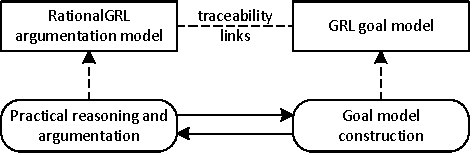
\includegraphics[scale=0.4]{img/framework}
\caption{The RationalGRL Framework}
\label{fig:rationalgrl-framework}
\end{figure}

We propose the following methodology (shown in Figure~\ref{fig:rationalgrl-methodology}) to develop an instance of the RationalGRL framework. Here we assume that the initial GRL models have been created based on the requirements specification documents and the discussions of the stakeholders. The rest of the steps are as follows:

\begin{figure*}[ht]
\centering

\includegraphics[scale=0.4]{img/methodology}
\caption{The RationalGRL Methodology}
\label{fig:rationalgrl-methodology}
\end{figure*}


\textbf{(1) Instantiate Argument Schemes (AS)} -- In this step, we start from the list of arguments schemes of the argumentation framework. We select an intentional element from the initial GRL model that we want to analyze and we instantiate a relevant argument scheme from the already existing list of argument schemes or by adding a new one. For example, an argument scheme can be "Goal \emph{G} contributes to softgoal \emph{S}". When an argument scheme is instantiated, it corresponds to  an argument for or against part of a goal model.

\textbf{(2) Answer Critical Questions (CQs)} -- After instantiating an argument scheme, we invoke related critical questions to attack the argument by counter-arguments.  Each argument scheme includes one or more critical questions. For example, for the argument scheme, "Goal \emph{G} contributes to softgoal \emph{S}", there are two critical questions as follows:  \emph{Does the goal contributes to the softgoal?} and \emph{Does the goal contributes to some other softgoals?}. 
%It is worth mentioning that, answering a critical question may result in a "conflict" situation. This is out of the scope of our work here.  
%MvZ: removed this sentence because I don't know what you mean with "conflict". I think We should explain it better or leave it out.
When the analyst answers  a critical question, a new argument scheme may be instantiated.  Thus, it is possible to go back and forth between this step and the step (1).

\textbf{(3) Decide on Intentional Elements and their Relationships} -- By answering a critical question, one of the four following cases can occur: \textsf{INTRO}, \textsf{DISABLE}, \textsf{REPLACE} or \textsf{ATTACK}.  Any of these cases can  impact the arguments and corresponding GRL intentional elements.  \textsf{INTRO} means that 
a new argument scheme is created. That means, the current argument scheme related to the critical question does not get attacked.  In the case of \textsf{DISABLE}, the intentional element or its related links are disabled or removed from the models. \textsf{REPLACE} introduces a new argument and attacks the original argument at the same time. This means that the original element of the argument scheme is replaced with a new one.   \textsf{ATTACK} is a generic counterargument which attacks any argument with another argument when new evidence occurs.  

\textbf{(4) Modify GRL Models} -- In this step, we modify the GRL models based on the situation of step (3). That is, one of the following situation can happen with respect to the initial GRL model: 1) a new intentional element or a new link is introduced; 2) an existing intentional element or an existing link gets disabled (removed) from the model; or 3) an existing intentional element or link is replaced by a new one. This results in a new modified GRL. The new GRL model can then impact the argument schemes and instantiate another argument scheme (Step (1)).   

We can continue these four steps until there is no more intentional element or link to analyze or we reach a satisfactory model. 

\subsection{Metamodel}

Figure~\ref{fig:metamodel} depicts the RationalGRL metamodel linking the main elements of our argumentation extension to the main GRL elements. We describe the metamodel bottom-up, starting with the GRL package.

The GRL package of our metamodel consists of the core GRL concepts, which constitute a part of
the URN metamodel from Recommendation Z.151~\cite{URN}. These concepts represent the abstract grammar of the language, independently of the notation. This metamodel also formalizes the GRL concepts and constructs introduced earlier\footnote{Note that for readability, some GRL concepts ave been omitted from the figure. For instance, a GRL contribution can have a qualitative strength, ranging from ``Make'' to ``Break''. Since these concepts are not relevant to our framework, they have been omitted, but none of the results of this article depend on this.}.

The GRL specification consists of \textsf{GRLModelElements}, which can be either \textsf{GRLLinkableElements} or \textsf{ElementLinks}. A \textsf{GRLLinkableElement} can again be specialized into an \textsf{Actor} or an \textsf{IntentionalElement} (which is either a \textsf{Softgoal}, \textsf{Goal}, \textsf{Task}, \textsf{Resource}, or a \textsf{Belief}). Intentional elements can be part of an actor, and \textsf{GRLLinkableElements} are connected through \textsf{ElementLinks} of different types (i.e., \textsf{Contribution, Decomposition}, or \textsf{Dependency}). Note that actors can be connected through links as well, which is done with \textsf{Dependency} links. 

The Argumentation package depicts the concepts we introduced in the previous sections. An \textsf{ArgumentScheme} represents an (uninstantiated) scheme containing variables that can be replaced with intentional elements. \textsf{CriticalQuestions} are possible ways to attack or elaborate an argument scheme. As such, each critical question applies to exactly one scheme, but each scheme can be elaborated or attacked through multiple critical questions. When an argument scheme is instantiated, we obtain an \textsf{Argument}. Therefore, each argument is associated with exactly one scheme, but a scheme can be instantiated in multiple ways. When a critical question is answered, we obtain an \textsf{AttackLink}. Each \textsf{AttackLink} is associated with at most one critical question, but a critical question can be used to attack multiple arguments.  Note that an \textsf{AttackLink} can also be associated with no critical questions. This allows the user to create attacks between arguments, which do not necessarily correspond to one of the critical questions. A \textsf{RationalGRLDiagram} is composed out of arguments and attack relations.

There is only one link between the \textsf{GRL} package and the \textsf{Argumentation} package, but it is a very important one. The link specifies that each \textsf{GRLModelElement} is in fact an argument. This means that each model element inherits the \textsf{AcceptStatus} as well, allowing GRL elements to be accepted, rejected, or undecided. This, furthermore, means that argument schemes can be applied to all GRL elements, capturing the intuition that each GRL element can be regarded as an instantiated argument scheme. Note that besides arguments about elements of the GRL model, we also have a \textsf{GenericArgument} which is simply a counter-argument to an existing argument that does not relate to any of the GRL elements, but can come from an external source, for instance a piece of evidence or an expert opinion. We will see various examples of such arguments in the next sections.

\begin{figure*}[h!]
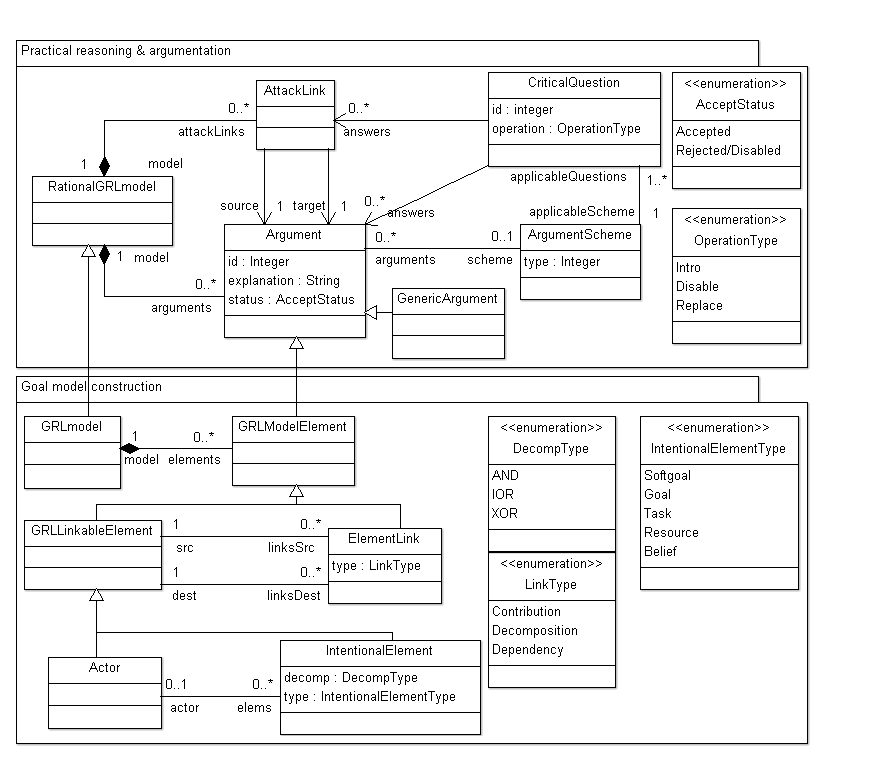
\includegraphics[width=\textwidth]{metamodel/metamodel}
\caption{The RationalGRL metamodel}
\label{fig:metamodel}
\end{figure*}